% Figure 3.2. Partial relaxation of vertex stress continuity at a 2D corner.
% Build in WSL: pdflatex for PDF, pdftocairo -eps for EPS, pdftocairo -png -r 300 for PNG.
\documentclass[tikz,border=3pt]{standalone}
\usepackage{amsmath}
\usepackage{tikz}
\usetikzlibrary{arrows.meta}

\begin{document}
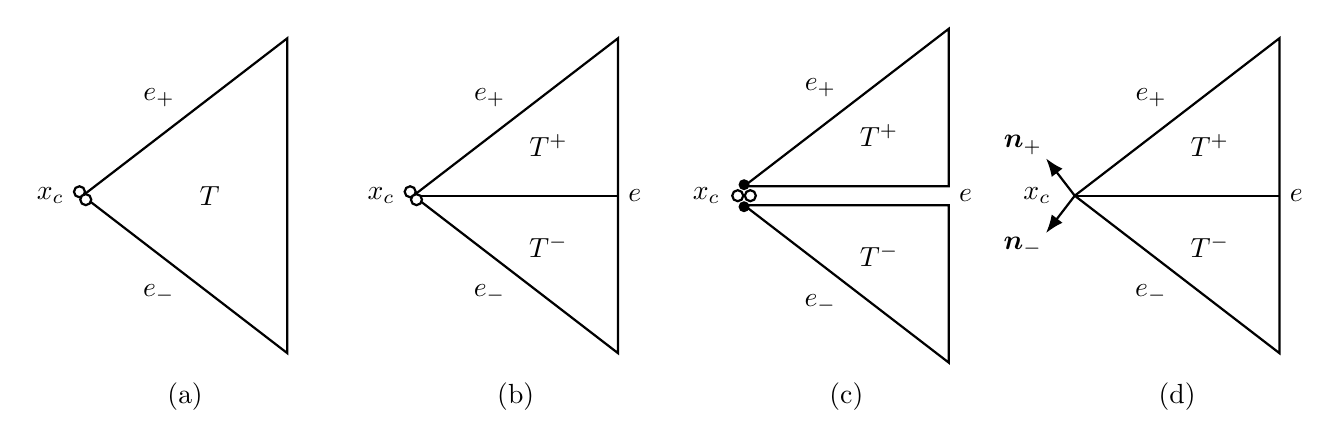
\begin{tikzpicture}[x=1cm,y=1cm,>=Latex,line width=0.8pt]
  \def\W{2.6}   % 三角形水平宽度
  \def\H{2.0}   % 三角形半高
  \def\G{4.2}   % 子图间距
  \def\R{0.07}  % 自由度圆点半径

  % ================= (a) 松弛前 =================
  \begin{scope}[shift={(0,0)}]
    \draw (0,0) -- (\W,\H) -- (\W,-\H) -- cycle;
    \draw[fill=white] (-0.04,0.05) circle (\R);
    \draw[fill=white] (0.04,-0.05) circle (\R);
    \node[left=3pt] at (0,0) {$x_c$};
    \node at (0.62*\W,0) {$T$};
    \node[above left] at (0.5*\W,0.5*\H) {$e_+$};
    \node[below left] at (0.5*\W,-0.5*\H) {$e_-$};
    \node at (0.5*\W,-\H-0.55) {(a)};
  \end{scope}

  % ================= (b) 划分为 T^+ 与 T^- =================
  \begin{scope}[shift={(\G,0)}]
    \draw (0,0) -- (\W,\H) -- (\W,-\H) -- cycle;
    \draw (0,0) -- (\W,0);
    \draw[fill=white] (-0.04,0.05) circle (\R);
    \draw[fill=white] (0.04,-0.05) circle (\R);
    \node[left=3pt] at (0,0) {$x_c$};
    \node[right] at (\W,0) {$e$};
    \node at (0.66*\W,0.32*\H) {$T^+$};
    \node at (0.66*\W,-0.32*\H) {$T^-$};
    \node[above left] at (0.5*\W,0.5*\H) {$e_+$};
    \node[below left] at (0.5*\W,-0.5*\H) {$e_-$};
    \node at (0.5*\W,-\H-0.55) {(b)};
  \end{scope}

  % ================= (c) 切向分量自由度拆分 =================
  \begin{scope}[shift={(2*\G,0)}]
    \def\d{0.12}
    \draw (0,\d) -- (\W,\H+\d) -- (\W,\d) -- cycle;
    \draw (0,-\d) -- (\W,-\H-\d) -- (\W,-\d) -- cycle;
    \fill (0,\d+0.02) circle (\R);
    \fill (0,-\d-0.02) circle (\R);
    \draw[fill=white] (-0.08,0) circle (\R);
    \draw[fill=white] (0.08,0) circle (\R);
    \node[left=5pt] at (0,0) {$x_c$};
    \node[right] at (\W,0) {$e$};
    \node at (0.66*\W,0.32*\H+\d) {$T^+$};
    \node at (0.66*\W,-0.32*\H-\d) {$T^-$};
    \node[above left] at (0.5*\W,0.5*\H+\d) {$e_+$};
    \node[below left] at (0.5*\W,-0.5*\H-\d) {$e_-$};
    \node at (0.5*\W,-\H-0.55) {(c)};
  \end{scope}

  % ================= (d) 松弛后：沿 e_+、e_- 的牵引自由度 =================
  \begin{scope}[shift={(3*\G,0)}]
    \draw (0,0) -- (\W,\H) -- (\W,-\H) -- cycle;
    \draw (0,0) -- (\W,0);
    % e_+ 与 e_- 的单位外法向
    \pgfmathsetmacro{\nx}{-\H/sqrt(\W*\W+\H*\H)}
    \pgfmathsetmacro{\ny}{\W/sqrt(\W*\W+\H*\H)}
    \draw[->] (0,0) -- (0.6*\nx,0.6*\ny) node[above left,inner sep=1pt] {$\boldsymbol{n}_+$};
    \draw[->] (0,0) -- (0.6*\nx,-0.6*\ny) node[below left,inner sep=1pt] {$\boldsymbol{n}_-$};
    \node[left=5pt] at (0,0) {$x_c$};
    \node[right] at (\W,0) {$e$};
    \node at (0.66*\W,0.32*\H) {$T^+$};
    \node at (0.66*\W,-0.32*\H) {$T^-$};
    \node[above left] at (0.5*\W,0.5*\H) {$e_+$};
    \node[below left] at (0.5*\W,-0.5*\H) {$e_-$};
    \node at (0.5*\W,-\H-0.55) {(d)};
  \end{scope}
\end{tikzpicture}
\end{document}
